\begin{figure}[t]
\centering
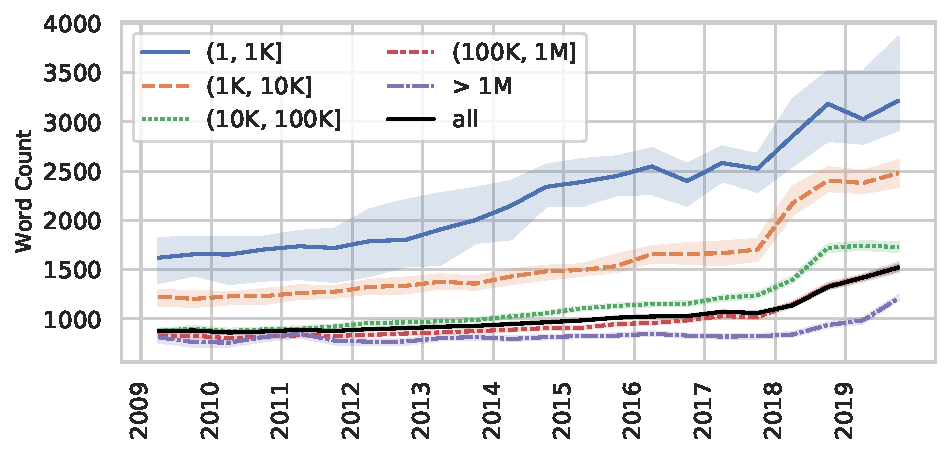
\includegraphics[width=0.99\columnwidth]{figures/word-count-by-rank.pdf}
\caption{The median word count of policies binned by Alexa rank. (The highlighted region in this and the following figures shows the 95\% confidence interval.)}
\label{fig:wordcount}
\end{figure}

\newcommand{\medianWCStartAlexa}{876}
\newcommand{\medianWCEnd}{1522}


{\bf Policy length.} Figure~\ref{fig:wordcount} shows the change in policy length as measured by word count. We see that the median word count has increased gradually over time---doubling between 2009A (\medianWCStartAlexa) and 2019B (\medianWCEnd) ---and more sharply in recent years, after the introduction of the GDPR; this trend holds for both popular and less popular websites. But the median hides a substantial variance: the 5\textsuperscript{th} percentile for word length is 248 words and the 95\textsuperscript{th} percentile is 3404 words. 
Our measurements for the top 10K are roughly consistent with the March 2016 measurements study by Degaling et al., but less so for their post-GDPR March 2018 measurements. Degaling et al. found the median privacy policy word count of the top 500 websites for 28 EU countries to be 2,145 (our data: 1K: 2,691, 10K: 2,122) and 3,044 (our data: 1K: 3,303, 10K: 2651) ~\cite{degeling2018we}. We believe the inconsistency is due to the difference in sampling.

